% Source p.1 (965). Heights below are visual layout only, not measured emissions.
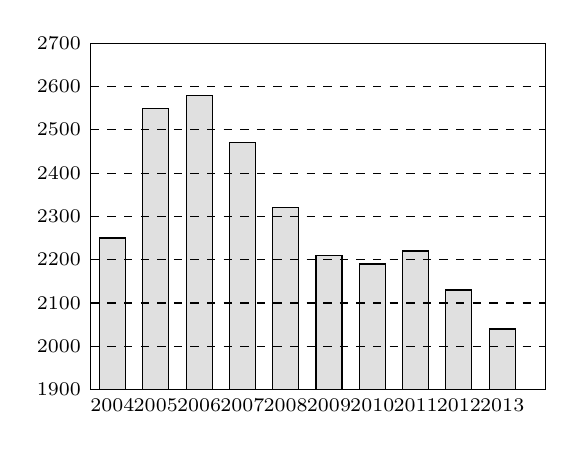
\begin{tikzpicture}[x=.55cm,y=.55cm,font=\scriptsize,line width=.4pt]
  \foreach \i/\h in {0/3.5,1/6.5,2/6.8,3/5.7,4/4.2,5/3.1,6/2.9,7/3.2,8/2.3,9/1.4}
    \draw[fill=black!12] (\i+.2,0) rectangle (\i+.8,\h);
  \foreach \j in {1,...,7} \draw[dashed] (0,\j)--(10.5,\j);
  \draw (0,0) rectangle (10.5,8);
  \foreach \j in {0,...,8} {
    \pgfmathtruncatemacro{\lab}{1900+100*\j}
    \node[left] at (0,\j) {\lab};
  }
  \foreach \i in {0,...,9} {
    \pgfmathtruncatemacro{\lab}{2004+\i}
    \node[below] at (\i+.5,0) {\lab};
  }
\end{tikzpicture}
